\section{Bill payment is received}
\label{scenario:bill-paid}

\npar Figure \ref{fig:scenario-5-14} shows the sequence diagram for the scenario
``Bill payment is received''.

\begin{figure}[H]
	\begin{centering}
		% TODO Figure
		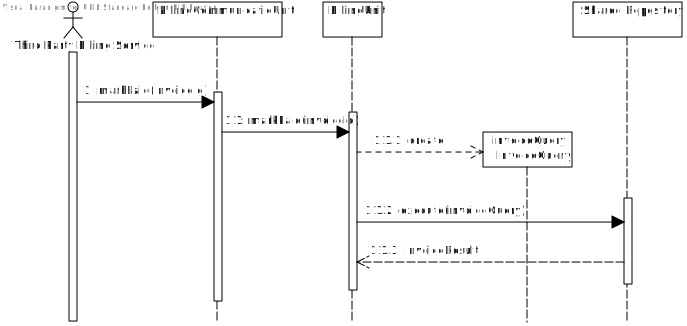
\includegraphics[width=\textwidth]{figs/scenario-5-14.pdf}
		\caption{Sequence diagram for the ``Bill payment is received'' scenario}
		\label{fig:scenario-5-14}
	\end{centering}
\end{figure}

\npar In step 1.1.1 of figure \ref{fig:scenario-5-14} an InvoiceQuery is
created. This query contains the invoiceId and the message that that invoice is
paid. The query is an update query, so the result that is returned
(InvoiceResult) will in fact be empty.
